% ============================================================
%  Présentation PFA – Commande Neuronale d'un Système Thermique à Distance
%  Beamer – visuel, centré sur les graphes
% ============================================================
\documentclass[aspectratio=169,12pt]{beamer}

% ---------- Encodage et langue ----------
\usepackage[utf8]{inputenc}
\usepackage[T1]{fontenc}
\usepackage[french]{babel}

% ---------- Packages ----------
\usepackage{amsmath,amssymb}
\usepackage{graphicx}
\usepackage{booktabs}
\usepackage{tikz}
\usetikzlibrary{arrows.meta,positioning,calc,shapes.geometric}
\usepackage{multicol}
\usepackage{xcolor}
\usetikzlibrary{calc}
% ---------- Thème ----------
%\usetheme{Madrid}
%\usecolortheme{whale}
\usetheme{default}
\usecolortheme{default}
% Couleurs ENIT
\definecolor{enitblue}{RGB}{0,51,102}
\definecolor{enitred}{RGB}{178,34,34}
\definecolor{enitgray}{RGB}{100,100,100}
\definecolor{lightblue}{RGB}{220,235,250}

\setbeamercolor{structure}{fg=blue}
\setbeamercolor{title}{fg=black,bg=white}
%\setbeamercolor{frametitle}{fg=white,bg=enitblue}
\setbeamercolor{frametitle}{fg=black, bg=white}
\setbeamercolor{block title}{bg=white,fg=black}
\setbeamercolor{block body}{bg=white,fg=black}
\setbeamercolor{item}{fg=black}
\setbeamercolor{block title alerted}{bg=enitred,fg=white}
\setbeamercolor{block body alerted}{bg=enitred!8,fg=black}
\setbeamercolor{block title example}{bg=green!40!black,fg=white}
\setbeamercolor{block body example}{bg=green!5,fg=black}

\setbeamerfont{title}{size=\large,series=\bfseries}
\setbeamerfont{frametitle}{size=\normalsize,series=\bfseries}

% Footer
\setbeamertemplate{footline}{%
	\leavevmode%
	\hbox{%
		\begin{beamercolorbox}[wd=.333333\paperwidth,ht=2.5ex,dp=1ex,center]{author in head/foot}%
			\usebeamerfont{author in head/foot}\insertshortauthor
		\end{beamercolorbox}%
		\begin{beamercolorbox}[wd=.333333\paperwidth,ht=2.5ex,dp=1ex,center]{title in head/foot}%
			\usebeamerfont{title in head/foot}\insertshorttitle
		\end{beamercolorbox}%
		\begin{beamercolorbox}[wd=.333333\paperwidth,ht=2.5ex,dp=1ex,right]{date in head/foot}%
			\usebeamerfont{date in head/foot}\insertshortdate{}\hspace*{2em}
			\insertframenumber{} / \inserttotalframenumber\hspace*{2ex}
	\end{beamercolorbox}}%
	\vskip0pt%
}
\setbeamertemplate{navigation symbols}{}

% Chemin des figures
\graphicspath{{figures/}}

% ---------- Infos ----------
\title[Commande Neuronale]{Commande Neuronale d'un Système Thermique à Distance}
\subtitle{Projet de Fin d'Année~II}
\author[Ouri \& Chaanbi]{Ouri Mohamed Amine \and Chaanbi Hassen}
\institute[ENIT]{ENIT -- Département Génie Électrique}
\date{2025/2026}

% ============================================================
\begin{document}
	
	% ============================================================
	% SLIDE 1 : Page de garde
	% ============================================================
	{
		\setbeamertemplate{footline}{}
		\begin{frame}[plain]
			\begin{tikzpicture}[remember picture,overlay]
				% Logo université (haut gauche)
				\node[anchor=north west] at ([xshift=0.5cm,yshift=-0.5cm]current page.north west) {
					
\includegraphics[height=1.5cm]{presentation/figures/fig_p1_1.png}
				};
				
				% Logo école d'ingénieurs (haut droite)
				\node[anchor=north east] at ([xshift=-0.5cm,yshift=-0.5cm]current page.north east) {
					
\includegraphics[height=1.7cm]{presentation/figures/fig_p1_2.png}
				};
			\end{tikzpicture}
			
			\vspace{1.5cm}
			
			% Bloc institution (centré)
			\begin{center}
				{\small
					République Tunisienne\\
					Ministère de l’Enseignement Supérieur et de la Recherche Scientifique\\
					Département Génie Électrique\\
					École Nationale d’Ingénieurs de Tunis}
			\end{center}
			
			\vspace{0.2cm}
			% Titre du projet
			\begin{center}
				\noindent\rule{0.8\textwidth}{1.5pt}\\[0.1cm]
				{\textbf{\Large Commande neuronale d'un système\\
						thermique à distance}}\\[0.1cm]
				
				\noindent\rule{0.8\textwidth}{2pt}\\[0.5cm]
				
				%{\large Présentation de soutenance}\\[0.3cm]
				%{\normalsize Projet de Fin d'Année 2ème année Génie Électrique}
			\end{center}
			\begin{center}
				\begin{tabular}{rl}
					\textbf{Étudiants :} & Ouri Mohamed Amine et Chaanbi Hassen \\[0.1cm]
					\textbf{Encadrant :} & M. Faouzi Bouani \\[0.1cm]
				\end{tabular}
			\end{center}
			\begin{center}
				\textbf{Année universitaire :} 2025/2026
			\end{center}
			\vfill
		\end{frame}
	}
	
	% ============================================================
	% SLIDE 2 : Plan
	% ============================================================
	\begin{frame}{\color{red} Plan de la présentation}
		\tableofcontents
	\end{frame}
	
	% ============================================================
	\section{Problématique et objectifs}
	% ============================================================
	\begin{frame}{\color{blue}I.Problématique et objectifs}		
		\begin{alertblock}{Le problème}
			Comment commander un système thermique \textbf{non linéaire}, 
			\textbf{de modéle inconnu} et \textbf{accessible à distance} ?
		\end{alertblock}
		\vspace{4pt}		
		\begin{itemize}
			\item PID $\rightarrow$ réglage difficile sans modèle précis
			\item Systèmes réels $\rightarrow$ non linéaires, perturbés
			\item Réglage empirique $\rightarrow$ instabilité possible
			\item Solution $\rightarrow$ \textbf{approches basées données (réseau de neurones)}
		\end{itemize}
	\end{frame}
	% SLIDE 3
	\begin{frame}{\color{red}Intérêt des réseaux de neurones}
		
		\begin{alertblock}{Pourquoi utiliser les RNA ?}
			Les réseaux de neurones permettent de commander des systèmes complexes 
			\textbf{sans modèle mathématique explicite}.
		\end{alertblock}
		
		\vspace{4pt}
		
		\begin{itemize}
			\item Approche basée sur les données expérimentales
			\item Capacité à approximer des systèmes \textbf{non linéaires}
			\item Adaptation aux variations et perturbations
			\item Réduction du besoin de modélisation analytique
		\end{itemize}
		
		\vspace{6pt}
		
		Apprentissage d’une loi de commande à partir des données :
		entrée/sortie du système
		
		
	\end{frame}
	% SLIDE 4:Développer commande PID:Fondements exemple d'application
	\begin{frame}{\color {red}Objectifs et démarche}
		\begin{center}
			\begin{tikzpicture}[scale=0.9, every node/.style={font=\small},
				phase/.style={draw=black, rounded corners=6pt, fill=white, 
					minimum height=14mm, minimum width=35mm, align=center, font=\small\bfseries}]
				\node[phase] (p1) at (0,0) {Théorie};
				\node[phase] (p2) at (5,0) {Simulations\\Matlab};
				\node[phase] (p3) at (10,0) {Validation \\expérimentale};
				\draw[-Stealth, thick, enitblue] (p1) -- (p2);
				\draw[-Stealth, thick, enitblue] (p2) -- (p3);
				
				%\node[font=\footnotesize, text=enitgray, below=3mm] at (p1.south) {Ch.~1};
				%\node[font=\footnotesize, text=enitgray, below=3mm] at (p2.south) {Ch.~2};
				%\node[font=\footnotesize, text=enitgray, below=3mm] at (p3.south) {Ch.~3};
			\end{tikzpicture}
		\end{center}
		
		\vspace{1pt}
		\begin{columns}[t]
			\column{0.3\textwidth}
			\begin{itemize}\small
				\item Etude des deux approches de commande
				\item Fondements théoriques
				\item Modélisation des systémes
			\end{itemize}
			\column{0.3\textwidth}
			\begin{itemize}\small
				\item Simulations  des deux commandes
				\item PID:Systéme du 1 et 2\textsuperscript{e} ordre
				\item  RNA:systéme non linéaire
				\item  Analyse des performances
			\end{itemize}
			\column{0.3\textwidth}
			\begin{itemize}\small
				\item Essai en boucle ouverte du systéme
				\item Extraction des données entrée-sortie
				\item Commande par esp32
				\item Commande à distance(ESP-NOW)
			\end{itemize}
		\end{columns}
	\end{frame}
	
	% ============================================================
	\section{Fondements théoriques}
	% ============================================================
	\begin{frame}{\color{blue}II.Fondements théoriques}
		\textbf{\color{red} Commande PID : principe}
		La commande PID (Proportionnelle - Intégrale - Dérivée) est une 
		méthode de régulation basée sur l’erreur entre la consigne et la sortie.
		
		
		\vspace{4pt}
		
		\begin{itemize}
			\item Erreur : $e(t) = r(t) - y(t)$
			\item Objectif : minimiser l’erreur et stabiliser le système
			\item Méthode simple et largement utilisée en industrie
		\end{itemize}
		
		\vspace{6pt}
		
		\begin{block}{Loi de commande}
			\[
			u(t) = K_p\,e(t) + K_i \int_{0}^{t} e(\tau)\,d\tau + K_d \frac{de(t)}{dt}
			\]
			\[
			u(k)=u(k-1)+c_0\,e(k)+c_1\,e(k-1)+c_2\,e(k-2)
			\]
		\end{block}
		
	\end{frame}
	\begin{frame}{\color{red}Effet des actions PID}
		
		\begin{itemize}
			\item \textbf{Action proportionnelle ($K_p$)}
			\begin{itemize}
				\item Réagit instantanément à l’erreur
				\item Améliore la rapidité
				\item Peut provoquer un dépassement
			\end{itemize}
			
			\vspace{4pt}
			
			\item \textbf{Action intégrale ($K_i$)}
			\begin{itemize}
				\item Élimine l’erreur statique
				\item Améliore la précision
				\item Peut ralentir le système
			\end{itemize}
			
			\vspace{3pt}
			
			\item \textbf{Action dérivée ($K_d$)}
			\begin{itemize}
				\item Anticipe les variations de l’erreur
				\item Améliore la stabilité
				\item Sensible au bruit
			\end{itemize}
			
		\end{itemize}
		
		\vspace{3pt}
		
		\begin{alertblock}{Limite}
			Le réglage des gains ($K_p, K_i, K_d$) reste délicat pour les systèmes non linéaires.
		\end{alertblock}
		
	\end{frame}
	% Exemple Systéme 2 éme ordre
	\begin{frame}{\color {red}Commande PID appliquée à un systéme de deuxiéme ordre}
		\begin{columns}[c]
			\column{0.34\textwidth}
			\small
			Fonction de transfert du système :
			$$H(s) = \dfrac{K_s\,\omega_0^2}{s^2+2\xi\omega_0\, s+\omega_0^2}$$
			
			\vspace{6pt}
			\begin{tabular}{lc}
				\toprule
				$K_s$      & 5 \\
				$\omega_0$ & 20 rad/s \\
				$\xi$      & 0,5 \\
				$T_e$      & 0,36 s \\
				\bottomrule
			\end{tabular}
			
			\vspace{8pt}
			{\footnotesize $\xi < 1$ : système sous-amorti $\Rightarrow$ présence de dépassement}
			
			\column{0.44\textwidth}
			\small
			Correcteur PID discrétisé :
			$$u(k) = c_0\,e(k) + c_1\,e(k-1) + c_2\,e(k-2) + u(k-1)$$
			
			\vspace{3pt}
			avec :
			$$c_0 = K_p\!\left(1+\frac{T_e}{T_i}+\frac{T_d}{T_e}\right)$$
			$$c_1 = -K_p\!\left(1+\frac{2T_d}{T_e}\right), \quad c_2 = K_p\frac{T_d}{T_e}$$
			
			\vspace{6pt}
			\begin{tabular}{lc}
				\toprule
				$c_0$ & 15 \\
				$c_1$ & 1  \\
				$c_2$ & 1  \\
				\bottomrule
			\end{tabular}
			
		\end{columns}
	\end{frame}
	%Simulation
	\begin{frame}{\color {red}Simulation PID -- Résultats en boucle fermée}
		\begin{center}
			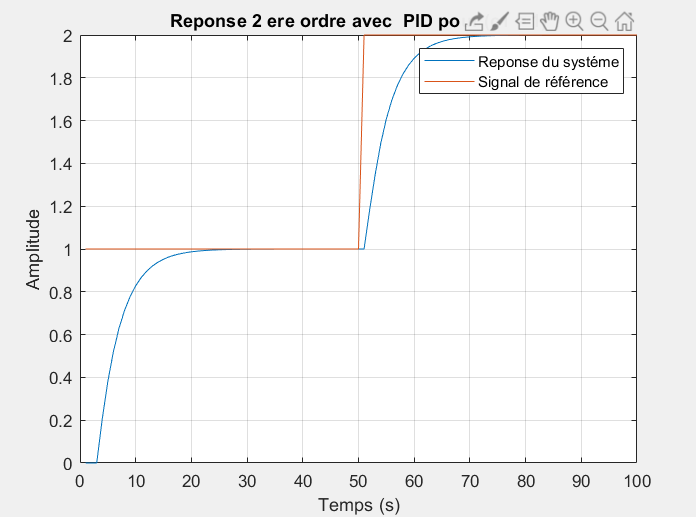
\includegraphics[height=0.55\textheight]{fig_p27_2.png}\hfill
			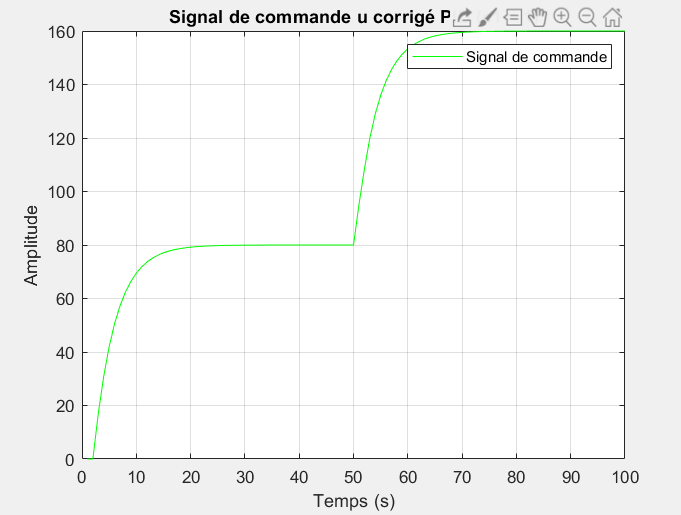
\includegraphics[height=0.55\textheight]{fig_p27_1.png}
		\end{center}
		\vspace{-2pt}
		{\footnotesize\centering (a) Réponse du systéme et la consigne \hspace{3cm} (b) Signal de commande $u(k)$\par}
		
		\vspace{4pt}
		\begin{center}
			\small $c_0=15,\; c_1=1,\; c_2=1$
			\quad \textbf{$\Rightarrow$Suivi correct avec erreur statique nulle}
		\end{center}
	\end{frame}
	%Commande NEURONALE
	%Slide1:Generalite
	\begin{frame}{\color {red}Réseaux de neurones}
		
		\begin{alertblock}{Principe}
			Un réseau de neurones (RNA) est un modèle mathématique capable 
			d’approximer des relations non linéaires à partir de données.
		\end{alertblock}
		
		\vspace{4pt}
		
		\begin{itemize}
			\item Approche basée sur les données (pas de modèle explicite)
			\item Approximation universelle des systèmes non linéaires
			\item Apprentissage à partir des couples entrée/sortie
			\item Utilisé comme modèle du système
		\end{itemize}
		
		\vspace{6pt}
		
		\begin{block}{Modélisation}
			\[
			\hat y(k) = NN\big(y(k-1),...,y(k-n),u(k-1),...u(k-m)\big)
			\]
		\end{block}
		
	\end{frame}
	%slide 2 Intéret
	\begin{frame}{\color {red}Intérêt des RNA}
		
		\begin{itemize}
			
			\item capable d'apprendre des relations complexes essentiellement avec les systémes \textbf{non linéaires}
			
			\item Ne nécessite pas de modèle analytique précis
			
			\item Capacité d’adaptation aux perturbations
			
			\item Utilisé comme \textbf{prédicteur} dans la boucle de commande
			
		\end{itemize}
		
		\vspace{6pt}
		
		\begin{alertblock}{Idée clé}
			Le RNA prédit la sortie future du système afin de calculer 
			une commande optimale.
		\end{alertblock}
		
	\end{frame}
	%Modéle du neurone artificiel ,et algorithme d'apprentissage
	\begin{frame}{\color{red} Neurone artificiel}
		
		\begin{columns}[c]
			
			\column{0.48\textwidth}
			\begin{center}
				\begin{tikzpicture}[scale=0.9, every node/.style={font=\small}]
					
					% Entrées
					\foreach \i/\label in {1/x_1, 2/x_2, 3/x_n} {
						\node[circle, draw, minimum size=6mm] (I\i) at (0, -\i*1.2+0.6) {$\label$};
					}
					\node at (0, -1.8) {$\vdots$};
					
					% Somme
					\node[circle, draw, minimum size=12mm] (N) at (3, -1.2) {$\Sigma$};
					
					% Activation
					\node[rectangle, draw, minimum height=8mm, minimum width=10mm] (A) at (5, -1.2) {$\varphi$};
					
					% Sortie
					\node (O) at (6.8, -1.2) {$y$};
					
					% Connexions
					\draw[-Stealth] (I1) -- node[above,font=\tiny]{$w_1$} (N);
					\draw[-Stealth] (I2) -- node[above,font=\tiny]{$w_2$} (N);
					\draw[-Stealth] (I3) -- node[below,font=\tiny]{$w_n$} (N);
					
					\draw[-Stealth] (N) -- (A);
					\draw[-Stealth] (A) -- (O);
					
					% Biais
					\node (B) at (3, 0.6) {$b$};
					\draw[-Stealth] (B) -- (N);
					
				\end{tikzpicture}
			\end{center}
			
			\column{0.5\textwidth}
			
			\begin{itemize}
				\item Combinaison linéaire des entrées
				\item Ajout d’un biais
				\item Fonction d’activation non linéaire
			\end{itemize}
			
			\vspace{6pt}
			
			\begin{block}{Modèle mathématique}
				\[
				y = \varphi\!\left(\sum_{i=1}^{n} w_i x_i + b \right)
				\]
			\end{block}
			
			\vspace{4pt}
			
			\begin{itemize}
				\item Exemple : $\varphi = \tanh$
			\end{itemize}
			
		\end{columns}
		
	\end{frame}
	\begin{frame}{\color{red}Modélisation neuronale du système}
		
		\begin{columns}[c]
			
			\column{0.55\textwidth}
			
			\begin{center}
				\begin{tikzpicture}[scale=0.9, every node/.style={font=\small},
					neuron/.style={circle, draw=black, minimum size=14mm},
					inp/.style={rectangle, draw=none}]
					
					\node[inp] (i1) at (0,  2.2) {$u(k-1)$};
					\node[inp] (i2) at (0,  0.8) {$y(k-1)$};
					\node[inp] (i3) at (0, -0.6) {$-1$};
					
					\node[neuron] (N) at (3.5, 0.8) {$\tanh$};
					
					\node[inp] (out) at (6.2, 0.8) {$\hat{y}(k)$};
					
					\draw[-Stealth, thick] (i1) -- node[above, sloped, font=\tiny]{$w_1$} (N);
					\draw[-Stealth, thick] (i2) -- node[above, font=\tiny]{$w_2$} (N);
					\draw[-Stealth, thick] (i3) -- node[below, sloped, font=\tiny]{$w_0$} (N);
					
					\draw[-Stealth, thick] (N) -- (out);
					
				\end{tikzpicture}
			\end{center}
			
			\column{0.4\textwidth}
			
			\begin{itemize}
				\item Modèle du système inconnu
				\item Entrées : $u(k-1)$, $y(k-1)$
				\item Sortie : $\hat{y}(k)$
				\item Approximation de la dynamique
			\end{itemize}
			
			\vspace{6pt}
			
			\begin{block}{Modèle}
				\[
				v(k) = -w_0 + w_1 u(k-1) + w_2 y(k-1)
				\]
				\[
				\hat{y}(k) = \tanh(v(k))
				\]
			\end{block}
			
		\end{columns}
		
	\end{frame}
	\begin{frame}{\color{red}Apprentissage du modèl neuronal:Identification du modéle neuronale du systéme}
		\begin{alertblock}{Objectif}
			Ajuster les poids du réseau pour minimiser l’erreur de prédiction
		\end{alertblock}
		\vspace{4pt}
		\begin{itemize}
			\item Données : $(u(k), y(k))$
			\item Prédiction : $\hat{y}(k+1)$
			\item Erreur :
			\[
			e(k+1) = y(k+1) - \hat{y}(k+1)
			\]
			\item Critère à minimiser:
			\[
			J = \frac{1}{2}\sum_{k = k_0}^{N} e(k+1)^2 =\frac{1}{2}\sum_{k = k_0}^{N}
			\left[y(k+1)-\tanh\big(-w_0 + w_1 u(k-1) + w_2 y(k-1)\big)
			\right]^2
			\]
		\end{itemize}	
	\end{frame}
	\begin{frame}
		\begin{itemize}
			\item Mise à jour des poids (descente de gradient) :
			\[
			w_i \leftarrow w_i - \eta \frac{\partial J}{\partial w_i}
			\]
		\end{itemize}
		\textbf{\color{green} $\eta$ : pas d'apprentissage}
	\end{frame}
	\begin{frame}{\color{red}Algorithme d'apprentissage du réseau de neurones (BGD)}
		\footnotesize
		
		\textbf{Entrées : $\{u(k),\, y(k)\}_{k=1}^{N}$ — Sortie : $w_0,\, w_1,\, w_2$}
		
		\begin{enumerate}\itemsep2pt
			\item Initialiser les poids $w_0,\, w_1,\, w_2$ 
			
			\item \textbf{Pour} chaque époque for $e = 1 \dots e_{\max}$ : {\color{green}"Boucle de passage"}
			\begin{enumerate}\itemsep1pt
				
				\item chaque échantillon de la donnée for $k =1 \dots N$ : {\color{green}" Boucle de mesure "}
				\[
				\hat{y}(k)=\tanh(-w_0+w_1u(k-1)+w_2y(k-1))
				\]
				
				\item Critère global :
				\[
				C_r=\frac{1}{N}\sum_{k=1}^{N}(y(k)-\hat{y}(k))^2
				\]
				
				\item Gradient :
				\[
				\frac{\partial C_r}{\partial w_j}
				=-\frac{2}{N}\sum_{k=1}^{N}(y(k)-\hat{y}(k))(1-\hat{y}(k)^2)\varphi_j(k)
				\]
				
				\item Mise à jour :
				\[
				w_j \leftarrow w_j - \mu_{\text{apprentissage}}\,\frac{\partial C_r}{\partial w_j}
				\]
				
			\end{enumerate}
			
			\item Arrêt : $C_r < \varepsilon$ ou $e = e_{\max}$
		\end{enumerate}
		
	\end{frame}
	%PRINCIPE DE LA COMMANDE PAR MV
	\begin{frame}{\color{red}Commande par Minimum de Variance}
		
		\begin{alertblock}{Objectif}
			Déterminer la commande $u(k)$ qui minimise l’erreur de poursuite.
		\end{alertblock}
		
		\vspace{4pt}
		
		\begin{itemize}
			
			\item Utilisation du RNA comme modèl prédictif
			
			\item Prédiction de la sortie future $\hat{y}(k+1)$
			
			\item Minimisation d’un critère de performance
			
		\end{itemize}
		
		\vspace{6pt}
		
	\end{frame}
	
	\begin{frame}{\color{red}Démarche de calcul de la commande par minimum de variance}
		
		Le critére :
		$$J = [y_c(k+1) - \hat{y}(k+1)]^2 + \lambda[u(k)-u(k-1)]^2$$
		La descente de gradient permet alors de :
		\begin{itemize}
			\item corriger \textbf{l'erreur de poursuite} par rapport à la consigne $e(k+1) = [y_c(k+1) - \hat{y}(k+1)]$
			\item \textbf{pénalise les variations brusques} de la commande.
		\end{itemize}
		Minimisation de la commande :
		$$u(k)_{i+1} = u(k)_i - \mu \frac{\partial J}{\partial u}$$
		
		avec $v = -w_0 + w_1\,u(k-1) + w_2\,y(k-1)$
		\quad et \quad $\hat{y}(k+1) = \tanh(v)$\\[6pt]	
	\end{frame}
	%Algorithme générale de commande par minimum de variance
	%\begin{frame}
	%Expression de la dérivation du critére de minimsation par rapport à la commande :
	%    $$\frac{\partial J}{\partial u} =\frac{\partial J}{\partial\hat{y}(k+1)}\frac{\partial\hat{y}(k+1)}{\partial v}\frac{\partial v}{\partial u} = 
	% -2\bigl[y_c(k+1) - \hat{y}(k+1)\bigr]\cdot w_1 \cdot\bigl(1 - \tanh^2(v)\bigr)
	%  +2\lambda\Delta u(k)$$, avec $\Delta u(k) = u(k)-u(k-1)$\\	
	%\end{frame}
	\begin{frame}{\color{red}Algorithme de commande par Minimum de Variance}
		\textbf{Entrées : $y(k),\, y_c(k+1),\, u(k-1)$ — Sortie : $u(k)$}
		\vspace{1pt}
		\begin{enumerate}
			\item Initialiser : $x \leftarrow u(k-1)$
			\item Calculer la prédiction courante :
			\[
			\hat{y}(k) = \tanh\bigl(-w_0 + w_1\,u(k-1) + w_2\,y(k-1)\bigr)
			\]
			\item \textbf{Pour} $i = 1 \dots i_{\max}$ :
			\begin{enumerate}
				\small
				\item Prédire la sortie future corrigée :
				\[
				\hat{y}(k+1) = \tanh(-w_0 + w_1\,x + w_2\,y(k)) + \alpha\bigl(y(k)-\hat{y}(k)\bigr)
				\]
				\item Calculer le gradient :
				\[
				\frac{\partial J}{\partial x} = -2\bigl(y_c(k+1)-\hat{y}(k+1)\bigr)(1-\tanh^2 v)\,w_1 + 2\lambda(x-u(k-1))
				\]
				\item Mettre à jour : $x \leftarrow x - \mu_{\text{commande}}\,\dfrac{\partial J}{\partial x}$
			\end{enumerate}
			%\item Saturer et appliquer : $u(k) = \mathrm{sat}_{[0,1]}(x)$
		\end{enumerate}
	\end{frame}
	\begin{frame}{Architecture de la commande neuronale avec optimsateur par minimum de variance}
		\begin{center}
			\begin{tikzpicture}[auto, node distance=2cm, >=Stealth, 
				block/.style={draw=black, fill=none, rectangle, minimum height=3em, minimum width=6em, line width=1pt, align=center, font=\small},
				optim/.style={draw=black, fill=none, rectangle, minimum height=3.5em, minimum width=8em, line width=1pt, align=center, font=\small},
				nn/.style={draw=black, fill=none, rectangle, minimum height=3em, minimum width=8em, line width=1pt, align=center, font=\small},
				val/.style={font=\footnotesize\itshape}]
				
				\node [coordinate] (input) {};
				
				\node [optim, right=1.5cm of input] (controller) {
					\textbf{Optimiseur Itératif}\\ 
					{\scriptsize Descente de gradient}\\
					{\tiny $i_{max}=10, \mu=0.1$}
				};
				
				\node [block, right=2.5cm of controller] (system) {
					\textbf{Système à commander           }\\
					{\scriptsize Pilote de puissance}
				};
				
				\node [coordinate, right=1.2cm of system] (output) {};
				
				\node [nn, below=1.8cm of system] (predictor) {
					\textbf{Modèle RNA $\hat{y}(k)$}\\
					{\scriptsize $\hat{y}(k+1) = \tanh(\mathbf{w}^T\mathbf{x}) + \alpha\cdot\text{err}$}
				};
				
				% --- Entrée yc ---
				\draw [->, thick, black] (input) -- node {$y_c(k+1)$} (controller);
				
				% --- u(k) : fil continu controller → system avec nœud au milieu ---
				\node [coordinate, right=1.25cm of controller] (uNode) {};
				\draw [->, thick, black] (controller) -- node[above]{$u(k)$} (system);
				
				% Point noir sur u(k) = nœud de distribution uniquement
				\node [circle, fill=black, inner sep=1.2pt] at (uNode) {};
				
				% --- u(k) → Modèle RNA ---
				\draw [->, thick, black] (uNode) |- (predictor.170);
				
				% --- y(k) : sortie système ---
				\draw [->, thick, black] (system) -- node[above]{$y(k)$} (output);
				
				% Point noir sur y(k) = nœud de distribution
				\node [circle, fill=black, inner sep=1.2pt] 
				at ($(system.east)+(0.6,0)$) (dotY) {};
				
				% --- y(k) → Modèle RNA ---
				\draw [->, thick, black] (dotY) |- (predictor.10);
				
				% --- y(k) → Optimiseur ---
				\draw [->, thick, black] (dotY) -- ++(0,-1.2) 
				-| (controller.south);
				
				% --- Sortie RNA : ŷ(k) sort à droite ---
				\node [coordinate, right=1.2cm of predictor] (outputRNA) {};
				\draw [thick, black] (predictor) -- node[above]{$\hat{y}(k)$} (outputRNA);
				
				% Point noir sur ŷ(k)
				\node [circle, fill=black, inner sep=1.2pt] at (outputRNA) (dotRNA) {};
				
				% Flèche continuation ŷ(k)
				\draw [->, thick, black] (outputRNA) -- ++(0.5,0);
				
				% --- ŷ(k) → Optimiseur ---
				\draw [->, thick, black] (dotRNA) -- ++(0,-0.8) 
				-| ([xshift=-1.5cm]controller.south);
				
				% --- Annotations ---
				\node [below=0.1cm of predictor, font=\tiny]
				{Modèle identifié du système thermique};
				\node [above=0.1cm of controller, font=\tiny]
				{Minimisation de la variance};
				
			\end{tikzpicture}
		\end{center}
	\end{frame}
	
	
	% ============================================================
	% SLIDE 6 : Architecture de commande (Optimisation par Gradient)
	% ============================================================
	% ============================================================
	%\section{Simulation et analyse}
	% ============================================================
	
	% SLIDE 7
	
	
	% SLIDE 8
	
	
	% SLIDE 9
	\begin{frame}{\color{red}Commande neuronale appliquée à un système non linéaire}
		\begin{block}{}
			\small $y(k) = -0{,}8\, y(k\!-\!2)\,\dfrac{[u(k\!-\!1)]^2}{1+[u(k\!-\!1)]^2} + 0{,}033\, y(k\!-\!1) + 0{,}5\, u(k\!-\!1)$
		\end{block}
		
		\vspace{2pt}
		\begin{columns}[c]
			\column{0.48\textwidth}
			\begin{center}
				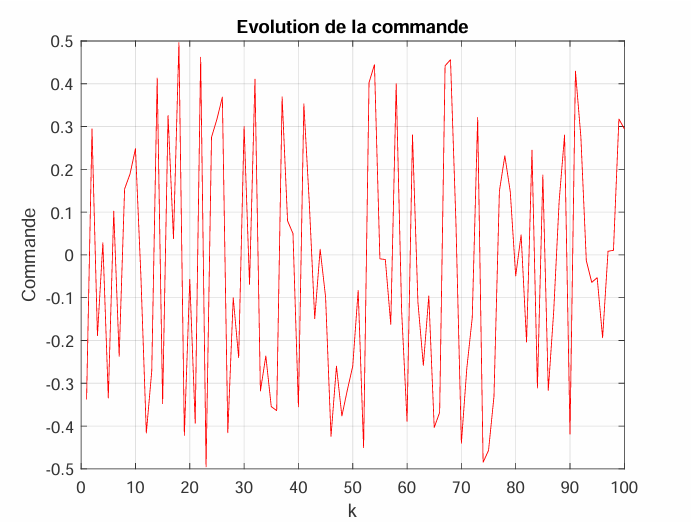
\includegraphics[width=\linewidth]{fig_p29_1.png}
			\end{center}
			%\vspace{-4pt}			
			\column{0.48\textwidth}
			\small
			\textbf{Topologie :}
			\begin{itemize}\footnotesize
				\item Entrées : $[-1,\; u(k\!-\!1),\; y(k\!-\!1)]^\top$
				\item Sortie : $\hat{y}(k) = \tanh(\mathbf{w}^\top\mathbf{x})$
			\end{itemize}
			\vspace{4pt}
			Non-linéarité + mémoire $(k\!-\!1, k\!-\!2)$
			\vspace{1pt}
			{\footnotesize\centering Commande aléatoire $u(k)\in[-0{,}5;\,0{,}5]$\par}
		\end{columns}
	\end{frame}
	
	% SLIDE 10
	\begin{frame}{\color{red}Résultats de l'identification neuronale:Phase d'apprentissage}
		\begin{figure}
			\centering
			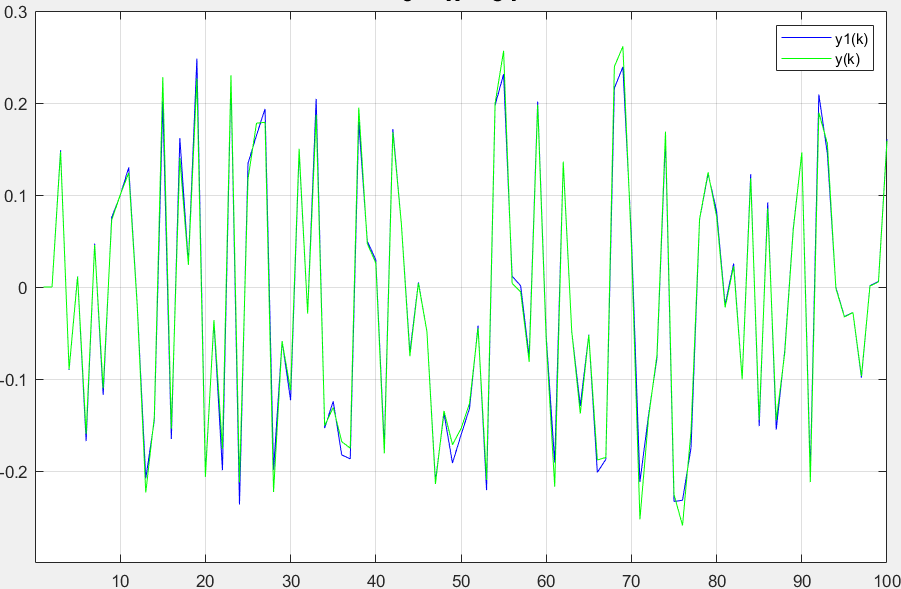
\includegraphics[width=0.75\linewidth]{figures/fig_p29_2}
			\caption{}
			\label{fig:figp292}
		\end{figure}
		
	\end{frame}
	\begin{frame}{\color{red}Résultats de l'identification neuronale : Convergence du critère $C_r$ (Descente de gradient \textbf{BGD})}
		\begin{center}
			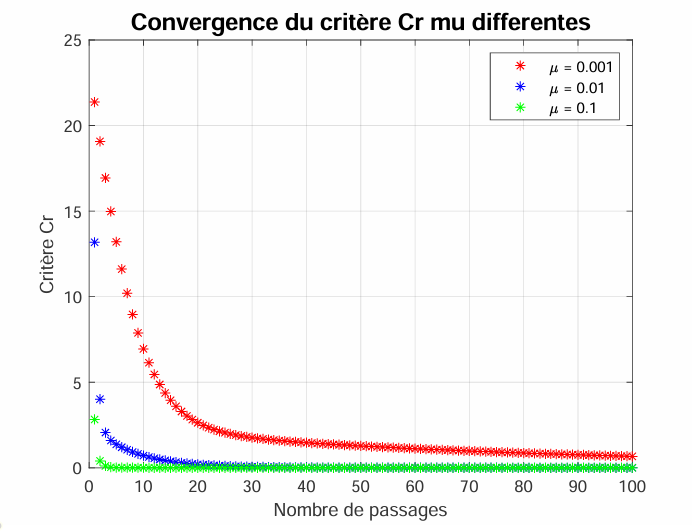
\includegraphics[height=0.75\textheight]{fig_p29_3.png}
			%\caption{}
		\end{center}
		{\footnotesize\centering Convergence du critère $C_r$ pour différents $\mu$\par}
	\end{frame}
	
	\begin{frame}{\color{red}Résultats de l'identification neuronale : Analyse de la convergence}
		\vspace{6pt}
		\begin{center}
			\small
			\begin{tabular}{ccc}
				\toprule
				$\mu$ & Comportement & Verdict \\
				\midrule
				0,001 & Très lent & Trop lent \\
				\textbf{0,01} & \textbf{Régulier} & \textbf{Optimal} \\
				0,1 & Rapide & Risque d'oscillations \\
				\bottomrule
			\end{tabular}
		\end{center}
		
		\vspace{8pt}
		\begin{block}{Paramètres identifiés (pour $\mu = 0{,}01$)}
			\[
			w_0 = -0{,}0442 \qquad w_1 = 0{,}0121 \qquad w_2 = 0{,}9369
			\]
		\end{block}
	\end{frame}
	%% ============================================================
	%  SLIDE A : Convergence du critère Cr
	%% ============================================================
	\begin{frame}{\color{red}Comparaison : Convergence du critère $C_r$}
		
		\begin{columns}[t]
			
			\column{0.48\textwidth}
			\begin{center}
				\textbf{1 Neurone}\\[4pt]
				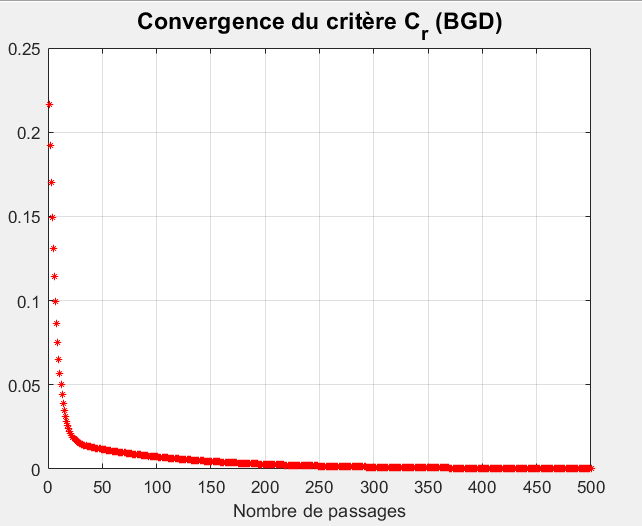
\includegraphics[width=\linewidth]{Cr_1.png}\\[2pt]
				{\tiny Convergence du critère $C_r$ -- 1 neurone}
			\end{center}
			\begin{itemize}\footnotesize
				\item Départ : $C_r \approx 0{,}22$
				\item Convergence \textbf{lente} : $\sim$200 passages
				\item Valeur finale élevée
				\item Capacité d'approximation \textbf{limitée}
			\end{itemize}
			
			\column{0.48\textwidth}
			\begin{center}
				\textbf{MLP -- 10 neurones cachés}\\[4pt]
				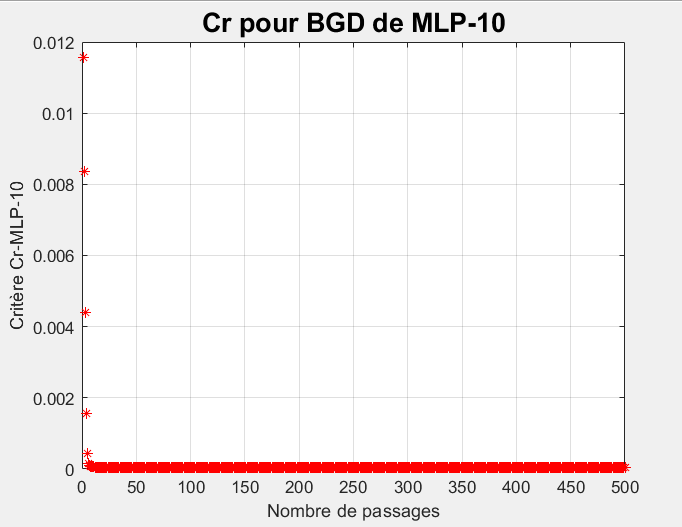
\includegraphics[width=\linewidth]{Cr_MLP_10.png}\\[2pt]
				{\tiny Convergence du critère $C_r$ -- MLP 10}
			\end{center}
			\begin{itemize}\footnotesize
				\item Départ : $C_r \approx 0{,}012$
				\item Convergence \textbf{rapide} : $\sim$15 passages
				\item Valeur finale quasi nulle
				\item Capacité d'approximation \textbf{supérieure}
			\end{itemize}
			
		\end{columns}
		
		\vspace{6pt}
		\begin{alertblock}{\centering Conclusion}
			\centering\small
			Le MLP-10 converge \textbf{10$\times$ plus vite} et atteint
			un critère \textbf{20$\times$ plus faible} que le neurone unique
			$\Rightarrow$ meilleure modélisation de la non-linéarité
		\end{alertblock}
		
	\end{frame}
	
	%% ============================================================
	%  SLIDE B : Erreur finale de test
	%% ============================================================
	\begin{frame}{\color{red}Comparaison : Erreur finale -- Phase de test}
		
		\begin{columns}[t]
			
			\column{0.48\textwidth}
			\begin{center}
				\textbf{1 Neurone}\\[4pt]
				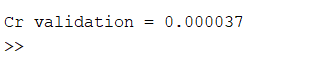
\includegraphics[width=\linewidth]{Test_1NN.png}\\[2pt]
				{\tiny Phase de test -- 1 neurone}
			\end{center}
			\begin{alertblock}{\centering\small Erreur de test}
				\centering
				$C_r^{\text{test}} \approx 2 \times 10^{-3}$\\[2pt]
				{\footnotesize
					\begin{itemize}
						\item Écart visible entre $y$ et $\hat{y}$
						\item Modèle \textbf{sous-paramétré}
						\item Ne capture pas la dynamique non linéaire
				\end{itemize}}
			\end{alertblock}
			
			\column{0.48\textwidth}
			\begin{center}
				\textbf{MLP -- 10 neurones cachés}\\[4pt]
				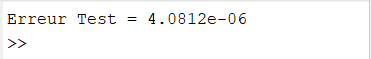
\includegraphics[width=\linewidth]{Test_10NN.png}\\[2pt]
				{\tiny Phase de test -- MLP 10 neurones}
			\end{center}
			\begin{exampleblock}{\centering\small Erreur de test}
				\centering
				$C_r^{\text{test}} = 4{,}08 \times 10^{-6}$\\[2pt]
				{\footnotesize
					\begin{itemize}
						\item Courbes $y$ et $\hat{y}$ \textbf{superposées}
						\item Bonne \textbf{généralisation}
						\item Dynamique non linéaire bien capturée
				\end{itemize}}
			\end{exampleblock}
			
		\end{columns}
		
		\vspace{4pt}
		\begin{center}
			\small
			Rapport d'erreur :
			$\dfrac{C_r^{\text{test}}(\text{1 neurone})}
			{C_r^{\text{test}}(\text{MLP-10})}
			\approx \mathbf{500}$
			\quad$\Rightarrow$\quad
			\textbf{le MLP-10 est indispensable pour ce système}
		\end{center}
		
	\end{frame}
	
	% SLIDE 11
	\begin{frame}{\color{red}Régulation : Application de la commande par minimum de variance au système : Test avec une consigne variable par palier}
		\begin{center}
			\vspace{8pt}
			\textbf{Optimisation itérative} ($i_{\max}=10$) :
			$$u_{\text{new}} = u_{\text{old}} - \mu\,\frac{\partial J}{\partial u}, \quad \mu = 0{,}2$$
			
			\vspace{10pt}
			\textbf{Remarque :}
			\[
			\mu_{\text{commande}} \neq \mu_{\text{apprentissage}}
			\]
			
			\vspace{10pt}
			$\lambda$ petit $\Rightarrow$ convergence rapide \quad\textbar\quad $\lambda$ grand $\Rightarrow$ convergence lente
		\end{center}
	\end{frame}
	
	% SLIDE 12
	\begin{frame}{\color{red}Commande min. variance pour les valeurs optimisées de $\lambda$ ($\lambda$ = 0.001)}
		\begin{columns}[c]
			\column{0.48\textwidth}
			\begin{center}
				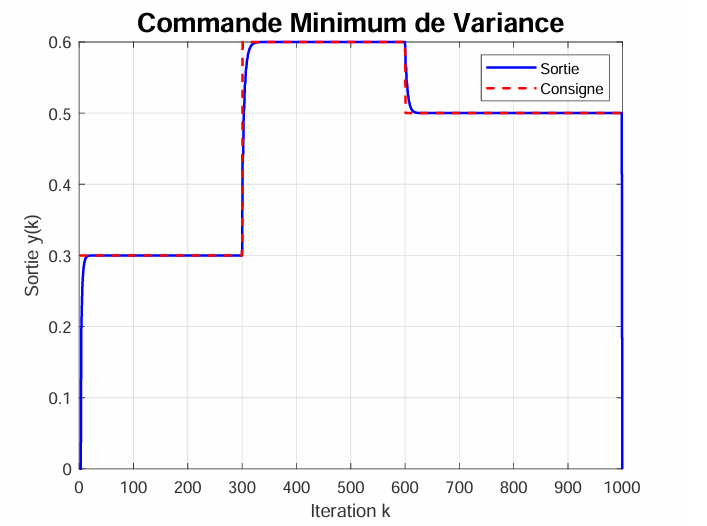
\includegraphics[width=\linewidth]{fig_p31_1.png}\\[4pt]
				{\footnotesize (a) Suivi de consigne}
			\end{center}
			
			\column{0.48\textwidth}
			\begin{center}
				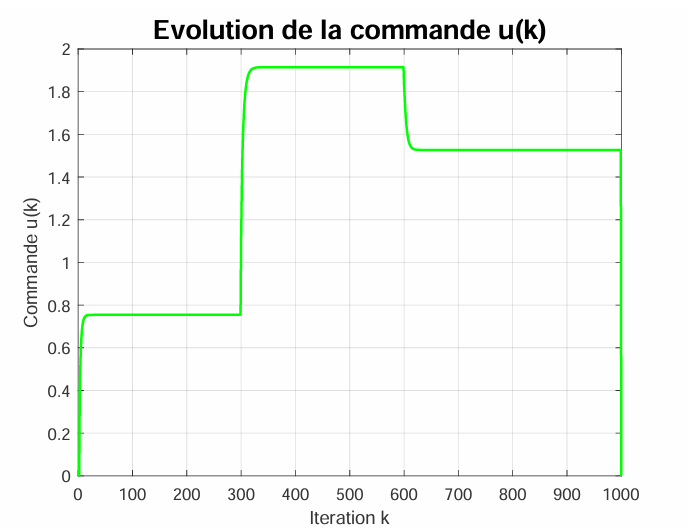
\includegraphics[width=\linewidth]{fig_p31_2.png}\\[4pt]
				{\footnotesize (b) Signal de commande $u(k)$}
			\end{center}
		\end{columns}
		
		\vspace{8pt}
		\begin{center}
			\small $\lambda$ faible $\Rightarrow$ \textbf{suivi rapide}, variations de commande acceptées
		\end{center}
	\end{frame}
	
	\begin{frame}{\color{red}Commande min. variance -- $\lambda = 4$}
		\begin{columns}[c]
			\column{0.48\textwidth}
			\begin{center}
				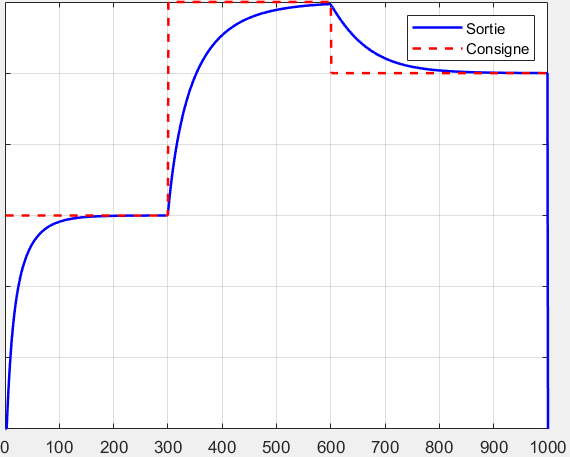
\includegraphics[width=\linewidth]{fig_p32_1.png}\\[4pt]
				{\footnotesize (c) Suivi de consigne dégradé}
			\end{center}
			
			\column{0.48\textwidth}
			\begin{center}
				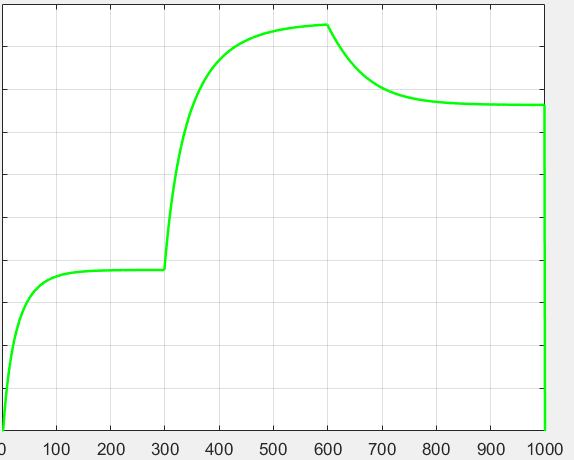
\includegraphics[width=\linewidth]{fig_p32_2.png}\\[4pt]
				{\footnotesize (d) Signal de commande $u(k)$}
			\end{center}
		\end{columns}
		
		\vspace{8pt}
		\begin{center}
			\small $\lambda = 4$ $\Rightarrow$ \textbf{commande lissée} mais suivi de consigne dégradé
		\end{center}
	\end{frame}
	
	% SLIDE 13
	%\begin{frame}{\color{red}Bilan des simulations}
	%Ici on va conclure sur les simulations obtneues ,pendant la démarche théorique quant'aux commande PID et commande par réseaux de neurones  
	%\end{frame}
	
	% ============================================================
	\section{Validation expérimentale}
	% ============================================================
	
	% SLIDE 14
	\begin{frame}{\color{blue}III.Validation expérimentale}
		\textbf{\color{red}Matériels de l'essai}
		\begin{columns}[c]
			\column{0.3\textwidth}
			\begin{center}
				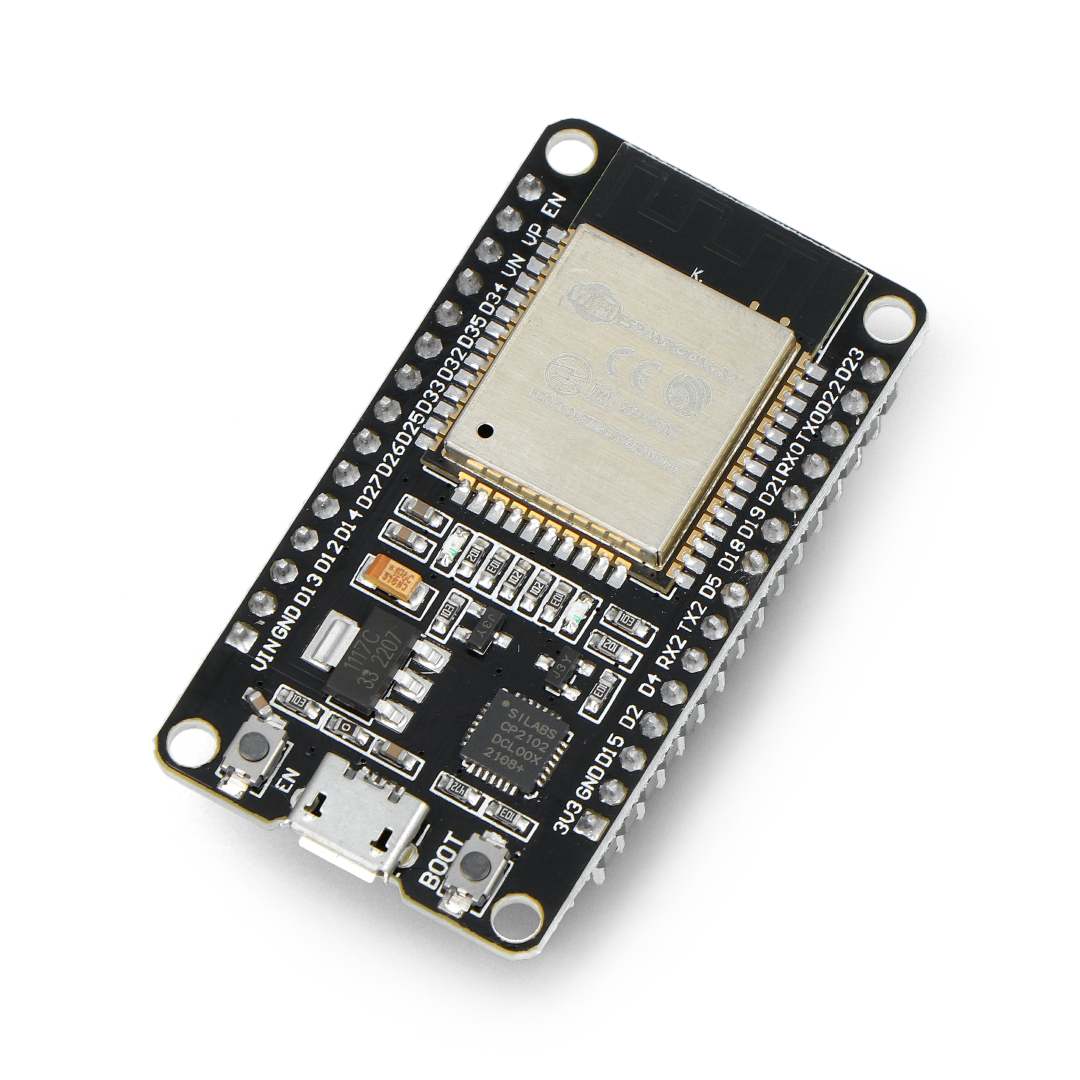
\includegraphics[width=0.85\linewidth]{fig_p34_1.jpeg}\\[2pt]
				{\footnotesize ESP32}
			\end{center}
			
			\column{0.3\textwidth}
			\begin{center}
				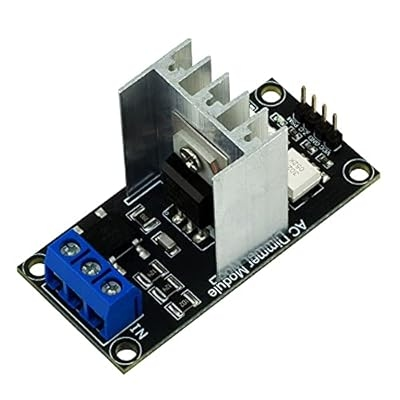
\includegraphics[width=0.7\linewidth]{fig_p36_1.jpeg}\\[2pt]
				{\footnotesize AC Dimmer}
			\end{center}
			
			\column{0.3\textwidth}
			\begin{center}
				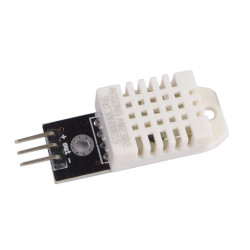
\includegraphics[width=0.65\linewidth]{fig_p36_2.jpeg}\\[2pt]
				{\footnotesize Capteur DHT22}
			\end{center}
		\end{columns}
		
		\vspace{8pt}
		\begin{center}
			\small
			\begin{tabular}{lccc}
				\toprule
				& \textbf{ESP32} & \textbf{Dimmer} & \textbf{DHT22} \\
				\midrule
				Rôle & Calcul \& comm. & Puissance AC & Mesure temp. \\
				Précision & -- & 8A, 220V & $\pm 0{,}1$°C \\
				\bottomrule
			\end{tabular}
		\end{center}
	\end{frame}
	
	% SLIDE 15
	\begin{frame}{\color{red}Architecture du système}
		\begin{center}
			\begin{tikzpicture}[scale=0.85, every node/.style={font=\small},
				block/.style={draw, rounded corners=4pt, minimum height=13mm, 
					minimum width=30mm, fill=white, text=black, 
					font=\small\bfseries, align=center},
				hw/.style={draw, rounded corners=4pt, minimum height=13mm, 
					minimum width=28mm, fill=white, font=\small, align=center}]
				% --- Nœuds ---
				\node[block, fill=white, text=enitred, minimum width=38mm] 
				(box)    at (0,    0)   {Boîte fermée\\{\tiny (enceinte thermique)}};
				\node[hw]    (dht)   at (-5,   0)   {DHT22\\{\tiny capteur}};
				\node[hw]    (lamp)  at ( 5,   0)   {Lampe 220V\\{\tiny source chaleur}};
				\node[block] (esp1)  at (-5,  -2.5) {ESP32\\mesure};
				\node[block] (esp2)  at ( 5,  -2.5) {ESP32\\commande};
				\node[hw]    (dimmer)at ( 5,  -4.5) {AC Dimmer\\(Modéle triac-gradateur)};
				
				% --- Connexions ---
				\draw[-Stealth, thick] (dht) -- (box);
				\draw[-Stealth, thick, enitred] (lamp) -- (box);
				
				\draw[-Stealth, thick] (dht) -- (esp1)
				node[midway, left]{\footnotesize temp.};
				
				\draw[Stealth-Stealth, ultra thick, enitblue, dashed] (esp1) -- (esp2)
				node[midway, below=2pt]{\footnotesize\textbf{ESP-NOW} (sans fil, 2.4~GHz)};
				
				\draw[-Stealth, thick] (esp2) -- (dimmer)
				node[midway, right]{\footnotesize PWM};
				
				% dimmer → lamp : passe par la droite pour éviter chevauchement
				\draw[-Stealth, thick] (dimmer.east) 
				-- ++(1.2, 0) 
				|- (lamp.east)
				node[pos=0.25, right]{\footnotesize puissance};
				
			\end{tikzpicture}
		\end{center}
	\end{frame}
	\begin{frame}{\color{red}Essai en boucle ouverte :Collecte de données}
		\begin{center}
			On lance un essai en boucle ouverte du système : le système est excité 
			par une commande variable $u(k)$ avec une période d'échantillonnage 
			$T_e = 2$~s, et la température est mesurée à chaque instant $k$.À l'issue de l'essai, on obtient une base de données expérimentale :
			
			\vspace{1pt}
			$$\mathcal{D} = \Big\{\,\big(u(k),\; y(k)\big),\quad k = 1, 2, \ldots, 2000\,\Big\}$$
			
			\vspace{2pt}
			\begin{itemize}
				\item $u(k)$ : commande appliquée à l'instant $k$
				\item $y(k)$ : température mesurée à l'instant $k$
				\item $T_e = 2$~s : période d'échantillonnage
				\item $N = 2000$ : nombre total d'échantillons
			\end{itemize}
			
			\vspace{6pt}
			$\Longrightarrow$ Cette base servira à \textbf{l'identification neuronale} du système.
		\end{center}
	\end{frame}
	\begin{frame}{\color{red}Essai en boucle ouverte :Collecte de données}
		\begin{columns}[c]
			\column{0.48\textwidth}
			\begin{center}
				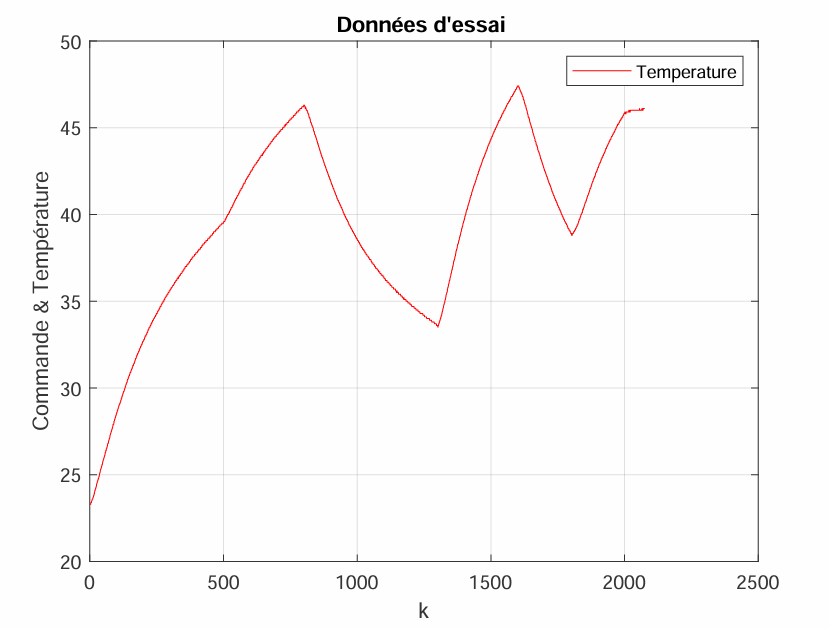
\includegraphics[width=\linewidth]{Temperature.png}
			\end{center}
			\vspace{-4pt}
			{\footnotesize\centering Température en fonction du temps\par}
			
			\column{0.48\textwidth}
			\begin{center}
				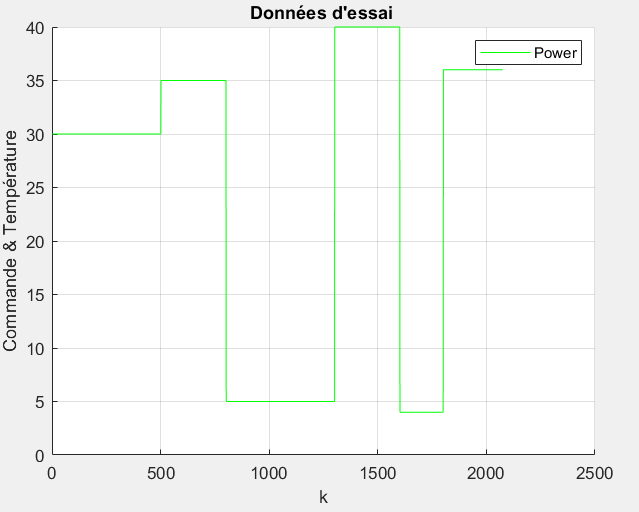
\includegraphics[width=\linewidth]{fig_p39_1.png}
			\end{center}
			\vspace{-4pt}
			{\footnotesize\centering Commande appliquée\par}
		\end{columns}
		
		%\vspace{6pt}
	\end{frame}
	
	% SLIDE 17
	\begin{frame}{\color{red}Apprentissage du neurone -- Phase d'entraînement}
		\begin{center}
			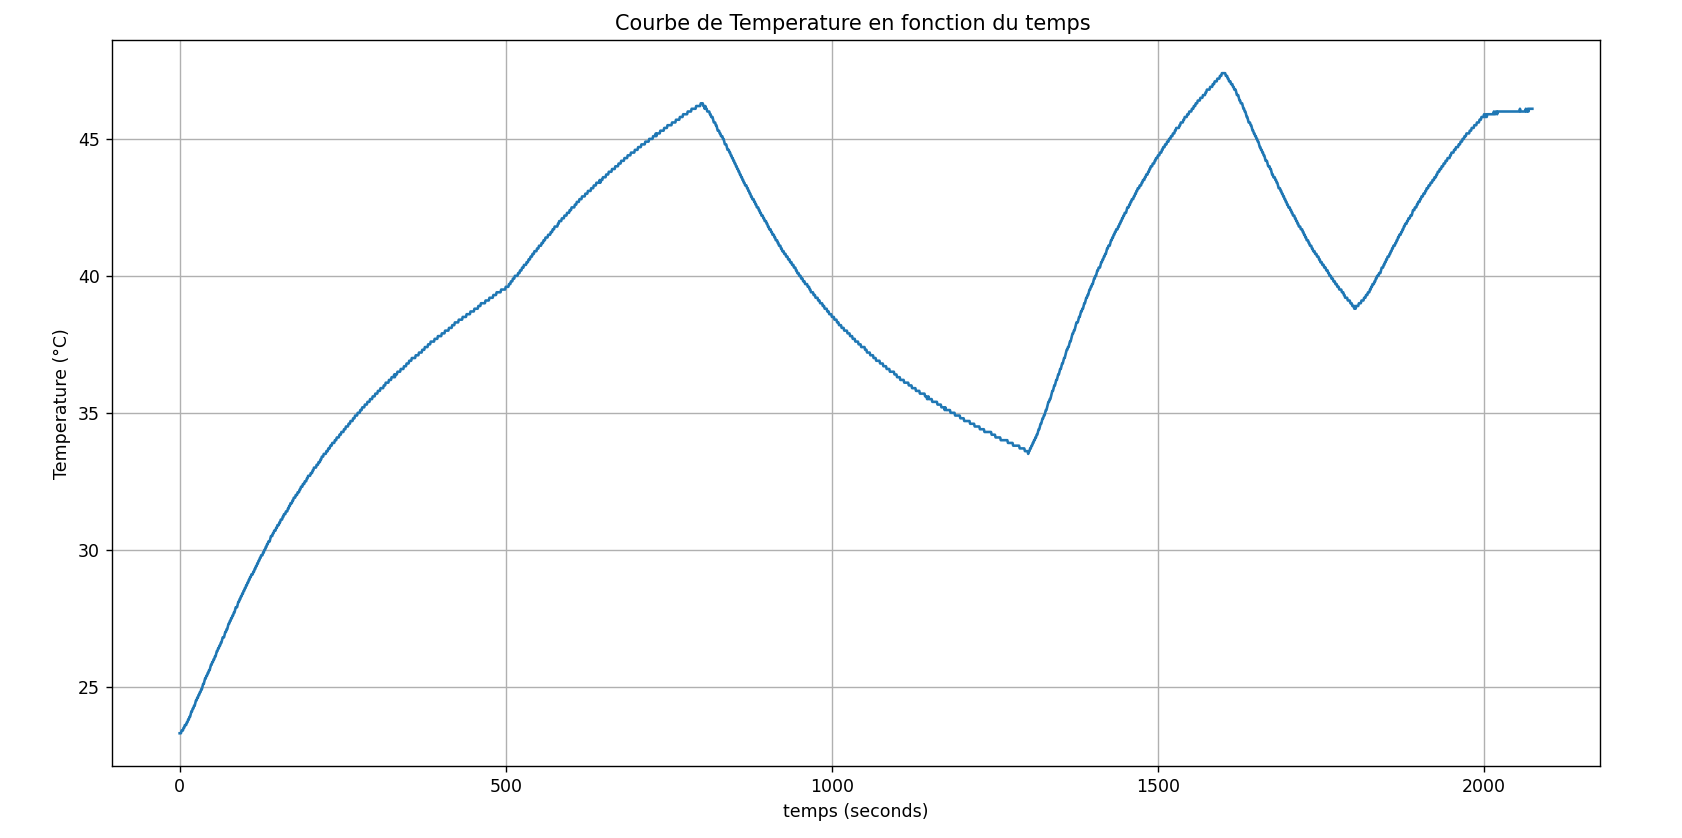
\includegraphics[height=0.65\textheight]{Apprentissage.png}
		\end{center}
		\vspace{-4pt}
		{\footnotesize\centering Sortie système vs sortie prédite du neurone -- \textbf{Phase d'apprentissage}\par}
		
		\vspace{4pt}
		\begin{center}
			\small Données normalisées ($T/100$, $u/5$) \quad\textbar\quad Descente de gradient itérative
		\end{center}
	\end{frame}
	
	% SLIDE 18
	\begin{frame}{\color{red}Apprentissage du neurone -- Phase de test}
		\begin{center}
			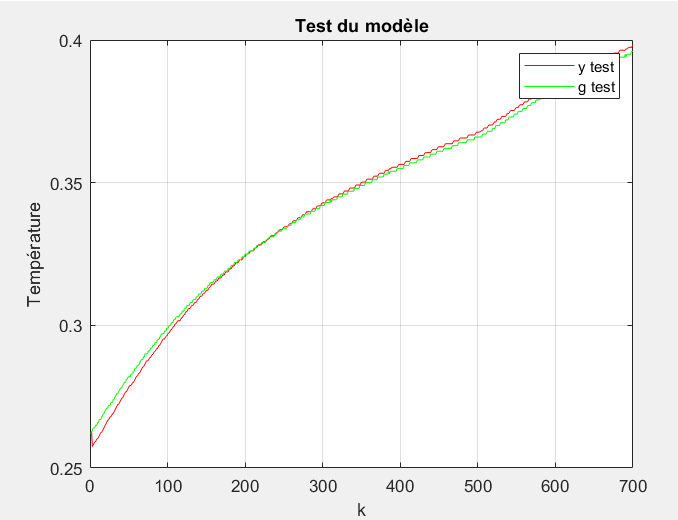
\includegraphics[height=0.65\textheight]{fig_p40_2.png}
		\end{center}
		\vspace{-4pt}
		{\footnotesize\centering Sortie système vs sortie prédite du neurone -- \textbf{Phase de test}\par}
		
		\vspace{4pt}
		\begin{center}
			\small Le modèle \textbf{généralise correctement} sur des données non vues $\Rightarrow$ poids validés
		\end{center}
	\end{frame}
	
	% SLIDE 19
	\begin{frame}{\color{red}Montage expérimental -- Boucle fermée}
		\begin{center}
			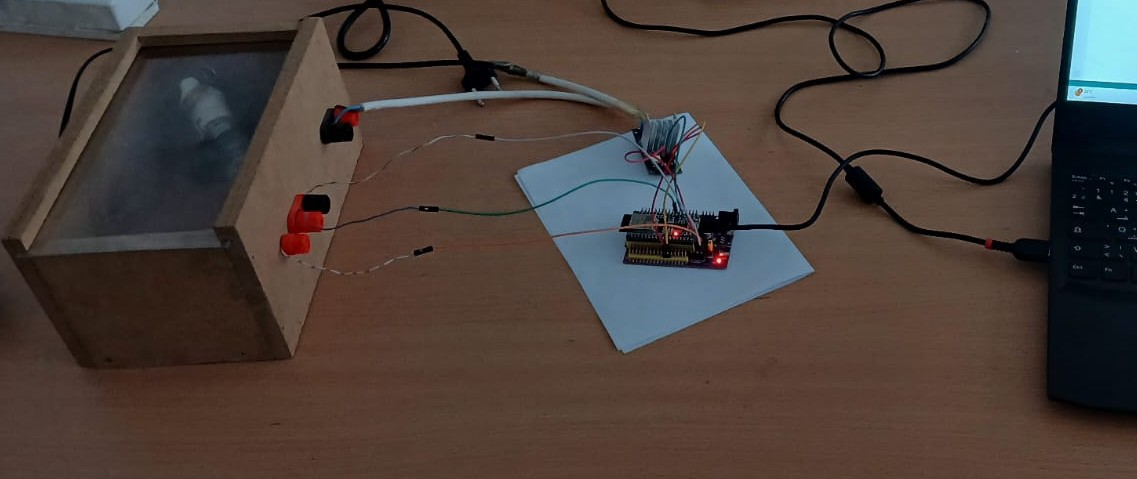
\includegraphics[height=0.7\textheight]{fig_p42_1.jpeg}
		\end{center}
		\vspace{-4pt}
		{\footnotesize\centering Montage : ESP32 + Dimmer + DHT22 + Lampe + Boîte fermée\par}
	\end{frame}
	
	% SLIDE 20
	\begin{frame}{\color{red}Résultats en boucle fermée -- Commande câblée}
		\begin{center}
			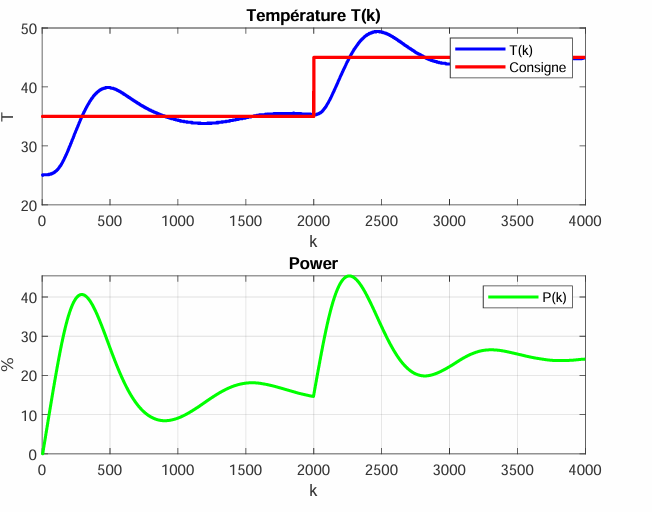
\includegraphics[height=0.62\textheight]{fig_p43_1.png}
		\end{center}
		\vspace{-4pt}
		{\footnotesize\centering Consigne 35°C puis 45°C -- 4000 échantillons -- Échantillonnage 2~s\par}
		
		\vspace{4pt}
		\begin{center}
			\small \textbf{La température suit la consigne} \quad\textbar\quad Oscillations faibles \quad\textbar\quad Système stable
		\end{center}
	\end{frame}
	
	% ============================================================
	\section{Communication sans fil}
	% ============================================================
	
	% SLIDE 21
	\begin{frame}{\color{blue}IV.Communication sans fil}
		\textbf{\color {red}Protocole ESP-NOW}
		\begin{columns}[c]
			\column{0.45\textwidth}
			\begin{center}
				\begin{tikzpicture}[scale=0.8, every node/.style={font=\footnotesize},
					card/.style={draw=enitblue, rounded corners=6pt, fill=lightblue, 
						minimum height=18mm, minimum width=30mm, align=center, font=\small\bfseries}]
					
					\node[card] (e1) at (0,0) {ESP32\\Commande};
					\node[card] (e2) at (5.5,0) {ESP32\\Mesure};
					
					\draw[-Stealth, ultra thick, enitred, dashed] 
					([yshift=3mm]e1.east) -- node[above]{\small Power } ([yshift=3mm]e2.west);
					
					\draw[-Stealth, ultra thick, enitblue, dashed] 
					([yshift=-3mm]e2.west) -- node[below]{\small Temp. } ([yshift=-3mm]e1.east);
					
					\node at (2.75, -1.5) {\small\textbf{2.4 GHz -- sans Wi-Fi}};
				\end{tikzpicture}
			\end{center}
			
			\column{0.45\textwidth}
			\begin{tabular}{ll}
				\toprule
				Fréquence & 2,4 GHz \\
				Latence & $\sim$ ms \\
				Portée & $\sim 200$ m \\
				Wi-Fi requis & Non \\
				Données max & 250 oct/trame \\
				\bottomrule
			\end{tabular}
		\end{columns}
	\end{frame}
	
	% SLIDE 22
	\begin{frame}{\color{red}Montage avec communication sans fil}
		\begin{center}
			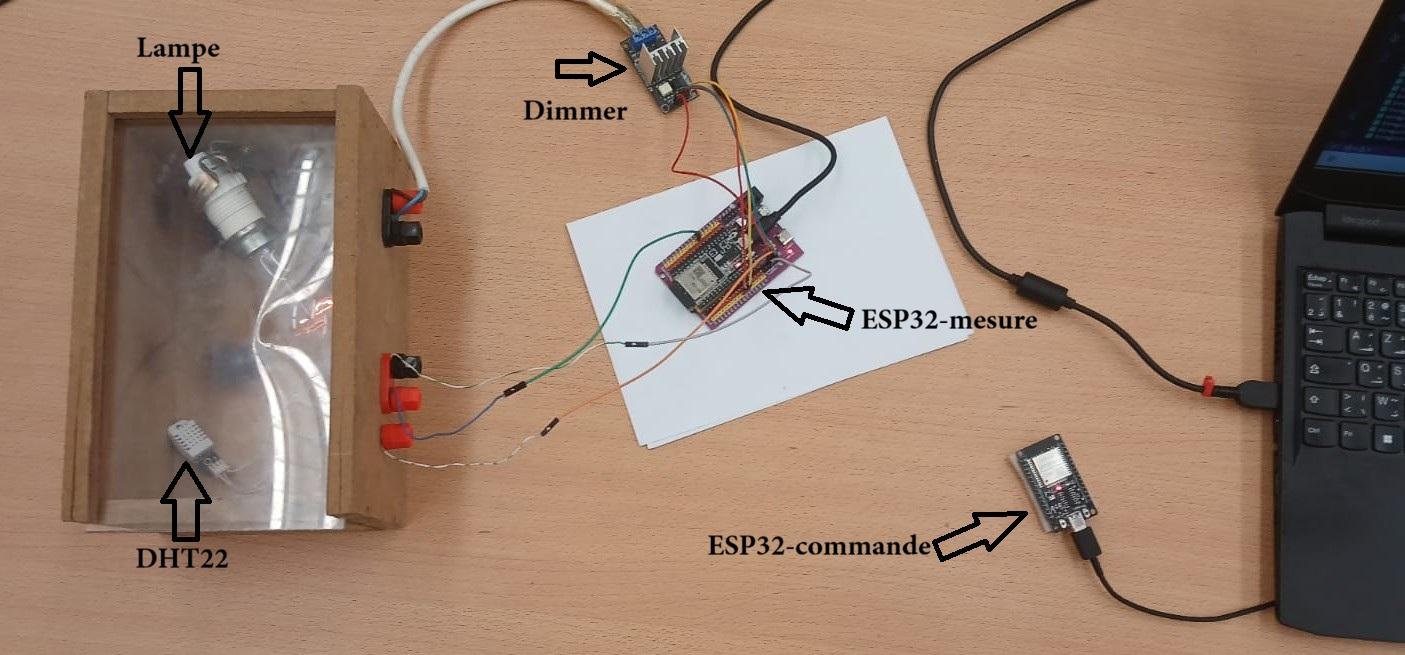
\includegraphics[height=0.7\textheight]{fig_p46_1.jpeg}
		\end{center}
		\vspace{-4pt}
		{\footnotesize\centering Montage expérimental avec 2 cartes ESP32 communicant via ESP-NOW\par}
	\end{frame}
	
	% SLIDE 23
	\begin{frame}{\color{red}Résultats -- Commande à distance}
		\begin{center}
			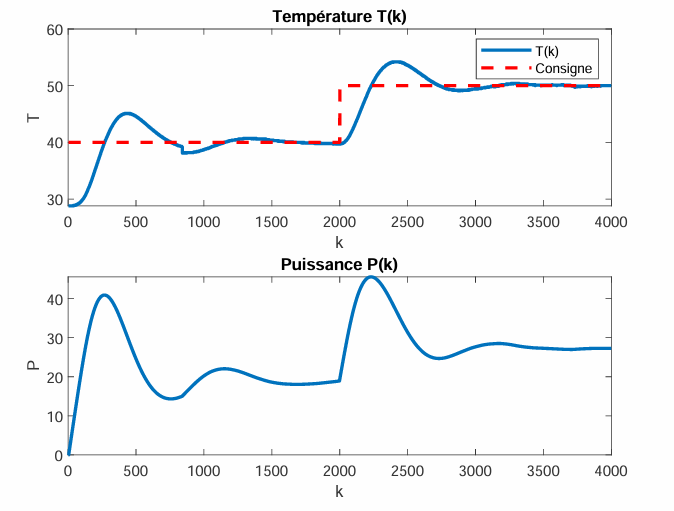
\includegraphics[height=0.62\textheight]{fig_p47_1.png}
		\end{center}
		\vspace{-4pt}
		{\footnotesize\centering Consignes : 40°C puis 50°C -- Communication sans fil ESP-NOW\par}
		
		\vspace{4pt}
		\begin{center}
			\small \textbf{Suivi de consigne confirmé} \quad\textbar\quad Retard dû à l'inertie thermique \quad\textbar\quad \textbf{Système stable}
		\end{center}
	\end{frame}
	
	% ============================================================
	\section{Bilan et conclusion}
	% ============================================================
	
	% SLIDE 24
	\begin{frame}{\color{blue}V.Bilan et conclusion}
		\textbf{\color{red}Bilan comparatif}
		\begin{center}
			\begin{tabular}{p{3.2cm}p{4cm}p{4.5cm}}
				\toprule
				\textbf{Critère} & \textbf{PID classique} & \textbf{Commande neuronale} \\
				\midrule
				Modèle requis & Oui (obligatoire) & \textbf{Non} \\
				Syst. linéaires & Très efficace & Efficace \\
				Syst. non linéaires & Inadapté & \textbf{Adapté} \\
				Réglage & Manuel & Automatique \\
				Adaptabilité & Faible & \textbf{Forte} \\
				\bottomrule
			\end{tabular}
		\end{center}
		
		\vspace{10pt}
		\begin{exampleblock}{Conclusion clé}
			\centering La commande neuronale est \textbf{complémentaire} au PID et \textbf{indispensable} pour les systèmes à modèle inconnu.
		\end{exampleblock}
	\end{frame}
	
	% SLIDE 25
	\begin{frame}{\color{red}Conclusion}
		\begin{columns}[c]
			\column{0.48\textwidth}
			\textbf{Ce qu'on a fait :}
			\begin{enumerate}\small
				\item Fondements théoriques (PID vs RNA)
				\item Simulations Matlab validées
				\item Implémentation sur ESP32
				\item Communication sans fil ESP-NOW
				\item Validation expérimentale réussie
			\end{enumerate}
			
			\column{0.48\textwidth}
			\textbf{Perspectives :}
			\begin{itemize}\small
				\item MLP multicouche plus profond
				\item Application à d'autres procédés industriels
				\item Commande prédictive neuronale
				\item Interface web de supervision
				\item Architectures avancées (LSTM)
			\end{itemize}
		\end{columns}
	\end{frame}
	
	
	
	% SLIDE FINALE : MERCI
	% ============================================================
	{
		\setbeamertemplate{footline}{}
		\begin{frame}[plain]
			\begin{tikzpicture}[remember picture,overlay]
				\fill[white] (current page.north west) rectangle (current page.south east);
			\end{tikzpicture}
			\vspace{2cm}
			\begin{center}
				{\color{black}\Huge\textbf{Merci de votre attention !}}\\[24pt]
			\end{center}
		\end{frame}
	}
	
	
	\begin{frame}{\color {red}Références et Bibliographie}
		\begin{thebibliography}{9}
			
			\bibitem{tlili2008}
			B. Tlili (2008).
			\textit{Modélisation et commande des systèmes électriques}.
			Thèse de doctorat, ENSAP.
			\url{https://theses.hal.science/tel00589735/file/THESE_B_TLILI_ACS_ENIT_2008.pdf}
			
			\bibitem{these1998}
			Auteur (1998).
			\textit{Méthodologie de modélisation et de commande par réseaux de neurones}.
			Thèse de doctorat, Université de Lille.
			\url{https://pepite-depot.univ-lille.fr/LIBRE/Th_Num/1998/50376-1998-309.pdf}
			\bibitem{ref4}
			K. Ben Saad (2020).
			\textit{Cours d'Automatique générale}, ENIT.
			\url{https://fr.scribd.com/document/493499963/cours-automatique-generale}
			
			\bibitem{ref5}
			J. Haggége (2012).
			\textit{Cours d'automatique}, ENIT.
			\url{https://fr.scribd.com/document/311533640/cours-automatique-pdf}
		\end{thebibliography}
	\end{frame}
	
	
	
	\begin{frame}{ }
		\begin{thebibliography}{9}
			\bibitem{ref6}
			M. Ould Moussa (2012).
			\textit{Modélisation du comportement dynamique non linéaire des structures en MMF}.
			Thèse de doctorat, École Polytechnique.\url{https://pastel.hal.science/pastel-00675919v1/file/modelisation_du_comportement_dynamique_des_MMFS.pdf}
			\bibitem{ref7}
			B.Faouzi(2026).
			\textit{Cours modélisation par réseaux de neurone artificiel},
			École nationale d'ingénieurs de Tunis.
			\bibitem{ref8}
			K.Zohra(2022/2023).
			\textit{Cours de l'automatique générale,introduction à la CNP}.
			Ecole nationale d'ingénieurs de Tunis.
			\url{https://drive.google.com/drive/folders/1VLzkrtT62niSaIGkrXEUMNOMCWhLwC2g}
			\bibitem{ref9}
			Claude Touzet(2016).
			\textit{Les réseaux de neurones artificiels, Introduction au connexionnisme}
			\url{https://amu.hal.science/hal-01338010/file/Les_reseaux_de_neurones_artificiels.pdf}
		\end{thebibliography}
	\end{frame}
	%\begin{frame}
	%	\begin{center}
		%		\color{blue}{\Huge Merci de votre attention}
		%	\end{center}
	%\end{frame}
	
	% ============================================================
	
	
\end{document}
